% !TEX root = Document.tex
\Chapter{Inspection d'infrastructure par UGV}
\label{sec:ugv}

Dans cette section nous présentons notre travail réalisé dans le cadre de l'article \textit{Motion Planning Strategy for the Active Vision-Based Mapping of Ground-Level Structures}.

\color{red}
Ajouter un breakdown des sections qui suivent.
\color{black}

\section{Description du problème} \label{sec:ugv_problem_description}
Une composante importante de tout système de SLAM est sa capacité de fermeture de boucle, c'est-à-dire d'être capable de reconnaître quand le robot retourne à un endroit déjà visité, particulièrement en l'absence de systèmes de positionenment absoluts. Ceci peut être fait localement sur un sous-ensemble local des observations courantes ou globalement sur toutes les observations faites jusqu'au présent. Ceci peut être réalisé d'une variété de façons dépendamment des capteurs utilisés par l'algorithme de SLAM. \citep{Hess2016} proposent Google Cartographer une approche hybride fonctionnant par scanner laser, où les nouveaux scans sont insérés et appariés par rapport à une sous-carte locale alors que la recherche de fermeture de boucle globale est exécutée en arrière plan par un algorithme de séparation et évaluation progressive (\textit{branch-and-bound}). En revanche RTAB-MAP \citep{Labbe2014} utilise une approche par sac-de-mots (\textit{bag-of-words}) appliquée à des descripteurs extraits d'une image couleur. Pour assurer une opération en temps réel les noeuds du graphe de pose, contenant aussi les mots visuels extraits à chaque endroit, sont séparés dans différentes mémoires: la mémoire court terme, la mémoire de travail et la mémoire long terme. Seuls les noeuds dans la mémoire de travail sont considérés pour la fermeture de boucle. Dans les deux cas de Google Cartographer et RTAB-MAP il est donc possible que la détection de la fermeture de boucle échoue si la pose estimée courante du robot a trop dérivé au point que les algorithmes ne cherchent plus à apparier l'environnement courant avec les éléments de la carte connue.

Le but de la fermeture de boucle est de réduire les erreures de localisation en imposant certaines contraintes sur la carte en cours de construction. Cette minimisation d'erreure peut-être réalisée de plusieurs façons, notamment par optimisation de graphe de poses \citep{Carlone2016}, par compensation par faisceaux (\textit{Bundle Adjustment}) \citep{Mei2011} ou tel que proposé dans ORB-SLAM2 une combinaison des deux \citep{Mur-Artal2017}.

C'est dans ce contexte que nous proposons une méthode de planification de trajectoire pour l'inspection de structures au sol cherchant à fermer la boucle le plus tôt possible pour d'une part augmenter les chances de succès de la détection de la fermeture de boucle et d'autre part minimiser les erreures de localisation. Pour ce faire, nous équipons un UGV d'un capteur de profondeur (une caméra) monté sur un joint à 1 degré de liberté en lacet ainsi que d'un scanner LIDAR permettant de détecter des obstacles dans un rayon de $180^\circ$ devant le véhicule.


% Plus spécifiquement étant donné une structure de taille finie et un robot équipé d'un capteur de profondeur mobile, nous cherchons à optimiser le positionnement de ce capteur pour cartographier la structure tout en maximisant la performance du système de SLAM.

\subsection{Hypothèses et fonctionnement de l'inspection}
\label{sec:ugv_hypothesis}

\textit{Hypothèse 1} L'inspection débute avec aucune information au préalable à propos de la structure. La caméra à bord du UGV est placé à une hauteur fixe $(0,0,h_c)$ par rapport à $\mathfs{R}$ et nous permet de recevoir une série de nuages de points combinées à des images RGB pour le système de SLAM visuel. Le système de SLAM à son tour nous fourni une carte 3D de l'environnement ainsi que notre trajectoire à travers celle-ci. Pour ce projet nous faisons spécifiquement usage de RTAB-Map \citep{Labbe2014} car c'est un système de SLAM à source ouverte mais nous soulignons que tout autre système de SLAM pourrait être utilisé pourvu qu'il fournisse l'information énoncé précedemment et que la détection de fermeture de boucle soit possible. Au départ de l'algorithme, l'UGV pointe la caméra vers sa droite face à l'un des murs de la structure.

\textit{Hypothèse 2} Soit une distance de sécurité $D$ devant être maintenue par rapport à la structure, nous supposons que l'espace se situant à $2D$ de la structure est libre d'obstacles. Ceci nous permettera à la section \ref{sec:perimeter_exploration} de savoir que les surfaces détectées par le LIDAR sont des extensions de la structure sous inspection.

\textit{Hypothèse 3} Finalement, nous supposons que la structure repose sur sur le plan horizontal $z^g = 0$. Ceci nous permet de simplifier certains de nos algorithmes pour filtrer le sol des nuages de points. Par extension, nous supposons aussi que la mission de l'UGV n'est que d'inspecter la partie de la structure visible dans le champ de vision de la caméra au sol. Ainsi, la hauteur maximale de la structure pouvant être cartographié est $H_{max} = h_c + D \tan{\psi/2}$ où $\psi$ est l'angle de vue vertical de la caméra.

\begin{table}[htp]
  \centering
  \setlength{\tabcolsep}{12pt}
  \begin{tabular}[htp]{|c|l|p{9cm}|}
    \hline
    Symbole & Nom                   & Description\\\hline
    $\mathsf{G} \coloneqq \{\mathsf{O_G}, \vect{x_g}, \vect{y_g}, \vect{z_g} \} $     &  \textit{Global}      & L'origine $\mathsf{O_G}$ se situant au point de départ du robot et les axes $\{\vect{x_g}, \vect{y_g}, \vect{z_g} \}$ alignés selon la pose initiale du robot.\\\hline
    $\mathsf{R} \coloneqq \{\mathsf{O_R}, \vect{x_r}, \vect{y_r}, \vect{z_r} \} $     &  \textit{Robot}       & Repère centré sur le robot avec les axes avant-gauche-haut.\\\hline
    $\mathsf{C} \coloneqq \{\mathsf{O_C}, \vect{x_c}, \vect{y_c}, \vect{z_c} \}$     &  \textit{Camera}      & Repère centré sur la caméra, la transformée est rigide par rapport à $R$ sauf pour l'angle de lacet. \\\hline
  \end{tabular}
  \setlength{\tabcolsep}{6pt}
  \caption{Repères présents dans le système d'inspections par UGV}
  \label{table:ugv_frames}
\end{table}

\begin{figure}[htp]
  \centering
  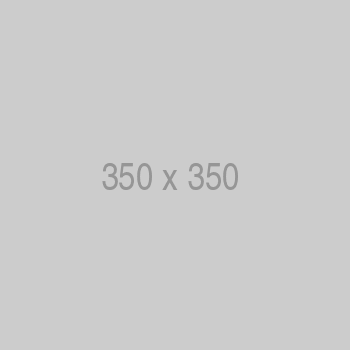
\includegraphics[width=0.3\linewidth]{images/placeholder.png}
  \caption{aa}
  \label{aa}
\end{figure}

L'inspection se fait en 2 phases, l'exploration du périmètre (EP) présentée dans la section \ref{sec:perimeter_exploration} suivit de l'exploration des cavités (EC) présentée dans la section \ref{sec:cavity_exploration}. Dans la première phase, l'UGV fait le tour de la structure en sautant les cavités pour fermer la boucle le plus tôt possible. Ensuite, une analyse de la carte 3D est effectuée pour trouver les \textit{frontier} indiquant des cavités non-explorées dans la structure. Une trajectoire est planifiée pour diriger le robot vers la cavité pour cartographier l'intérieur de la structure. L'inspection se termine quand toutes les cavités ont été inspectées.

\section{Exploration du périmètre} \label{sec:perimeter_exploration}

Suivant les hypothèses de la section \ref{sec:ugv_hypothesis} le problème d'inspection se simplifie au parcours de la partie de la structure située entre les plans $z^g = 0$ et $z^g = H_{max}$. Pour ce faire la phase EP débute avec le robot près de l'un des murs de la structure. Le robot parcours le périmèetre dans le sens horaire gardant toujours une partie visible de la structure dans son champ de vision vers sa droite. À chaque itération de l'algorithme, l'UGV détermine la prochaine pose objectif auquel se rendre pour placer la caméra à une distance $D$ perpendiculairement à la surface de la structure, maximisant ainsi al qualité des détails perçus et la densité des points captés.

\subsection{Choix de la prochaine pose objectif}

L'algorithme \ref{alg:PE_next_goal} présente la méthode par laquelle nous calculons la prochaine pose objectif, permettant à l'UGV de suivre la surface de la structure. Étant donné un nuage de point $\mathca{P}$ provenant de la caméra, nous filtrons d'abord le sol en éliminant tous les points sous une certaine hauteur $z^g = s$. Ensuite à la ligne \ref{alg:slice:decoupe}, nous découpons $\mathca{P}$ pour obtenir un sous ensemble $\mathca{S}$ adjacent à la prochaine section à inspecter, c'est-à-dire que $\mathca{S}$ est une partie (nous choisissons $1/3$) de $\mathca{P}$ vers la gauche de la caméra. Plus formellement, $\mathca{S}$ est choisi tel que les coordonnées en $y^c$ des points qui le compose satisfont
\begin{align}
  y^c_{max} - \frac{y^c_{max} - y^c_{min}}{3} \leq y^c \leq y^c_{max}
\end{align}
où $y^c_{max}$ et $y^c_{min}$ sont le maximum et le minimum des coordonnées $y^c$ de $\mathcal{P}$.

La \ref{alg:slice:pca}\textsuperscript{ième} étape est de déterminer la normale $\vect{n}$ de la surface. \citep{Rusu2009} explique que par le passé ceci aurait été fait en résolvant un problème des moindres carrés pour ajuster le modèle d'un plan au nuage $\mathcal{S}$. On peut représenter le plan par un point $\vect{x}$ et un vecteur normal $\vect{n}$, et la distance d'un point $\vect{p}_i \in \mathcal{S}$ au plan est défini par $d_i = (\vect{p}_i - \vect{x} \cdot \vect{n})$. On choisi $\vect{x} = \vect{p}^c$ la moyenne des points de $\mathcal{S}$.
\begin{align}
  \vect{x} = \vect{p}^c = \frac{1}{k} \cdot \sum^{k}_{i=1} \vect{p}_i
\end{align}

Suivant une formulation par moindres carrés on cherche donc à mettre les $d_i = 0$. La solution de $\vect{n}$ peut être trouvée par Analyse des Composantes Principales (ACP) en calculant les vecteurs propres et les valeurs propres de la matrice de covariance $\mathcal{C} \in \mathbb{R}^{3\times 3}$ de $\mathcal{S}$.
\begin{align}
  \mathcal{C} = \frac{1}{k} \sum^{k}_{i=1} (\vect{p}_i - \vect{p}^c) \cdot (\vect{p}_i - \vect{p}^c)^\top, \mathcal{C} \cdot \vect{v}_j = \lambda_j \cdot \vect{v}_j, j \in \{0, 1, 2\}
\end{align}
Où \mathcal{C} est semi-défini positive et les valeurs propres $\lambda_j \in \mathbb{R}$. Les vecteurs propres $\vect{v}_j$ forment ainsi une base orthonormale correspondantes aux composantes principales de $\mathcal{S}$. En classant les valeurs propres par $0 \leq \lambda_3 \leq \lambda_2 \leq \lambda_1$, nous avons $\vect{v}_3$ le vecteur propre correspondant à la plus petite valeur propre $\lambda_3$ qui est donc une approximation de la normale $\pm \vect{n} \sim \vect{v}_{3}$ du plan mais avec un ambiguïté de signe.

\begin{algorithm}[ht]
  \SetAlgoLined
  \SetKwData{Left}{left}\SetKwData{This}{this}\SetKwData{Up}{up}
  \SetKwFunction{Union}{Union}\SetKwFunction{FindCompress}{FindCompress}
  \SetKwInOut{Input}{entrée}\SetKwInOut{Output}{sortie}
  \Input{$\mathcal P$ Le nuage de point provenant de la caméra}
  \Input{$\alpha$ La longueur de pas à parcourir à chaque itération}
  \Input{$D$ La distance à garder par rapport aux murs}
  \Output{${po}$ la position objectif de la caméra}
  \Output{$\vect{u}$ le vecteur d'orientation de la caméra}

  $\mathcal S$  $\gets$ FiltrageDuSol($\mathcal P$)   \\
  $\mathcal S$  $\gets$ DécoupeAvant($\mathcal S$) \label{alg:slice:decoupe}   \\
  $\vect{p}^c$         $\gets$ Moyenne($\mathcal S$)         \\
  $[\vect{v}_1, \vect{v}_2, \vect{v}_3; \lambda_1, \lambda_2, \lambda_3] \gets$ AnalyseComposantesPrincipales($\mathcal S$) \label{alg:slice:pca}\\
  $\vect{\tilde u} \gets \vect{v}_3 - (\vect{v}_3\cdot\vect{z}_{\fr c})\vect{v}_3 $ \tcc{Projection vers le plan $\vect{x_c}\vect{y_c}$} \\
  $\vect{u} \gets \vect{\tilde u} \; \text{sign}(\vect{\tilde u} \cdot \overrightarrow{O_{\fr c} \overline{p}^{\fr c}}); \vect{u} \gets \vect{u}/\|\vect{u}\|$ \label{alg:slice:sign} \\
  $\vect{r} \gets \vect{z}_{\fr c} \times \vect{u}$ \\
  ${po} \gets p^c - D \vect{u} + \alpha \vect{r}$     \\
  \Return ${po}, \vect{u}$

  \caption{Calcul de la prochaine pose objectif au moyen du nuage de point courant de la caméra.}
  \label{alg:PE_next_goal}
\end{algorithm}

Le vecteur normal $\vect{v}_3$ est projetté sur le plan $\vect{x}_c\vect{y}_c$ sur lequel repose la caméra et pour résoudre l'ambiguïté de signe possible provenant de $\vect{v}_3$, $\vect{u}$ est pris pour pointer dans la direction du vecteur $\overrightarrow{O_{\fr c} \overline{p}^{\fr c}}$, c'est-à-dire de la caméra au centre de $\mathcal{S}$. L'algorithme retourne aussi la position objectif ${po}$ de la caméra dans $\mathsf{G}$

\subsection{Planification de trajectoire locale}

\subsection{Replanification pour le saut de cavités}

\subsection{Fin de l'exploration de périmètre}

\section{Exploration des cavités} \label{sec:cavity_exploration}

\section{Résultats} \label{sec:ugv_results}

\section{Conclusion et travail futur}
